% generated by scripts/pkl_to_latex.py
% source PKL : vscan_v1_L6_Ne6_U10_t1_mode-uniform_nmin2_solver-gcg_full_restarts10_iter300_kmax5_tol1em09_V0to12_N25-ebabade1a2a1.pkl
% scan type  : vscan
% state      : gs
% quantity   : cgme
% requires   : \usepackage{pgfplots} \pgfplotsset{compat=1.18}
% colours match the matplotlib PDF (tab10 cycle)
\definecolor{gmeC0}{HTML}{1F77B4}
\definecolor{gmeC1}{HTML}{FF7F0E}
\definecolor{gmeC2}{HTML}{2CA02C}
\definecolor{gmeC3}{HTML}{D62728}
\definecolor{gmeC4}{HTML}{9467BD}
\definecolor{gmeC5}{HTML}{8C564B}
\definecolor{gmeC6}{HTML}{E377C2}
\definecolor{gmeC7}{HTML}{17BECF}

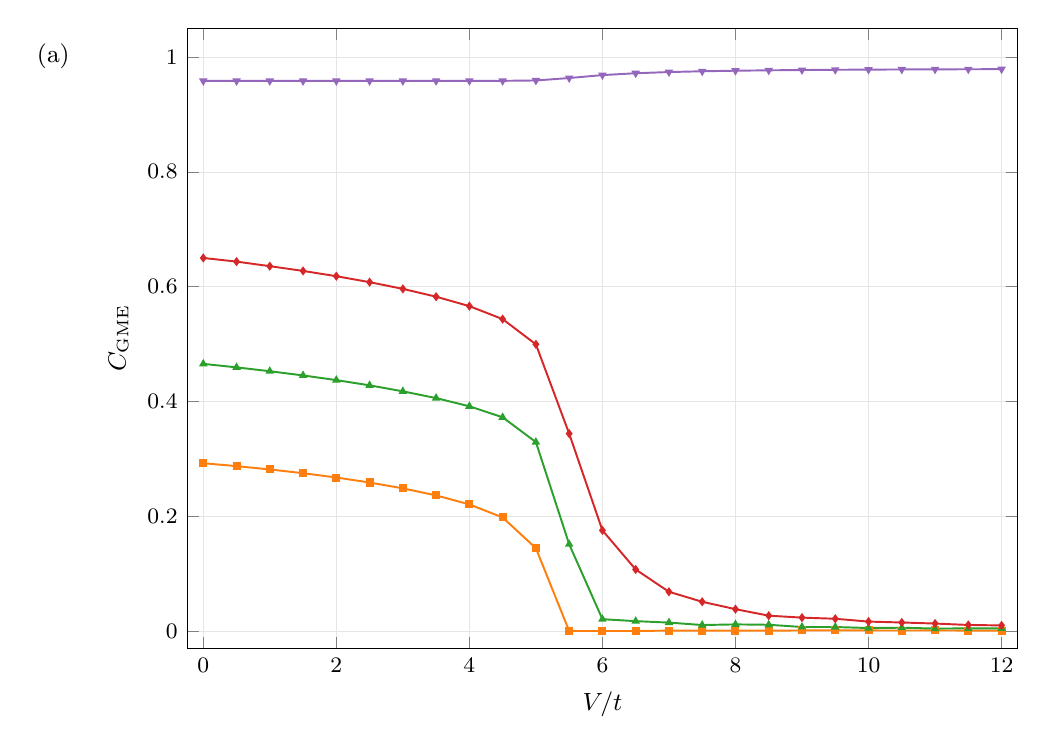
\begin{tikzpicture}
  \begin{axis}[
    width=\columnwidth,
    height=0.78\columnwidth,
    xlabel={$V/t$},
    ylabel={$C_{\mathrm{GME}}$},
    grid=both,
    grid style={line width=.1pt, draw=gray!20},
    tick label style={font=\footnotesize\rmfamily, /pgf/number format/fixed},
    label style={font=\small\rmfamily},
    scaled ticks=false,
    legend style={font=\scriptsize\rmfamily, draw=gray!40, at={(0.5,1.03)}, anchor=south, /tikz/every even column/.append style={column sep=6pt}},
    legend cell align={left},
    legend columns=2,
    ymin=-0.03,
    ymax=1.05,
    xmin=-0.24,
    xmax=12.24,
    after end axis/.append code={\node[anchor=east, font=\small\rmfamily] at (axis description cs:-0.13,0.954) {(a)};},
  ]
    \addplot[color=gmeC1, mark=square*, mark size=1.1pt, line width=0.7pt] coordinates {
        (0,0.292503) (0.5,0.287397) (1,0.281631) (1.5,0.27508)
        (2,0.267581) (2.5,0.258905) (3,0.248713) (3.5,0.236422)
        (4,0.220801) (4.5,0.198035) (5,0.144459) (5.5,0.000281)
        (6,0.000327) (6.5,0.00031) (7,0.000965) (7.5,0.001082)
        (8,0.000941) (8.5,0.000888) (9,0.00123) (9.5,0.001358)
        (10,0.00127) (10.5,0.001119) (11,0.001314) (11.5,0.001008)
        (12,0.000784)
    };
    \addplot[color=gmeC2, mark=triangle*, mark size=1.1pt, line width=0.7pt] coordinates {
        (0,0.465509) (0.5,0.459404) (1,0.45268) (1.5,0.445355)
        (2,0.437196) (2.5,0.428108) (3,0.417651) (3.5,0.405869)
        (4,0.391657) (4.5,0.372443) (5,0.32929) (5.5,0.151359)
        (6,0.020854) (6.5,0.017436) (7,0.014949) (7.5,0.010673)
        (8,0.011789) (8.5,0.011152) (9,0.007273) (9.5,0.007224)
        (10,0.005468) (10.5,0.006013) (11,0.004557) (11.5,0.004848)
        (12,0.004808)
    };
    \addplot[color=gmeC3, mark=diamond*, mark size=1.1pt, line width=0.7pt] coordinates {
        (0,0.649928) (0.5,0.643564) (1,0.635627) (1.5,0.627347)
        (2,0.618138) (2.5,0.607807) (3,0.596072) (3.5,0.582465)
        (4,0.566042) (4.5,0.543437) (5,0.499459) (5.5,0.344018)
        (6,0.175507) (6.5,0.10743) (7,0.068587) (7.5,0.051179)
        (8,0.038341) (8.5,0.026996) (9,0.023594) (9.5,0.021615)
        (10,0.016672) (10.5,0.015136) (11,0.013259) (11.5,0.010821)
        (12,0.010003)
    };
    \addplot[color=gmeC4, mark=triangle*, mark size=1.1pt, mark options={rotate=180}, line width=0.7pt] coordinates {
        (0,0.958182) (0.5,0.958184) (1,0.958185) (1.5,0.958187)
        (2,0.958191) (2.5,0.958197) (3,0.958207) (3.5,0.958226)
        (4,0.958267) (4.5,0.958382) (5,0.95901) (5.5,0.963252)
        (6,0.968364) (6.5,0.971607) (7,0.973662) (7.5,0.975034)
        (8,0.975992) (8.5,0.976688) (9,0.977209) (9.5,0.977609)
        (10,0.977923) (10.5,0.978174) (11,0.978378) (11.5,0.978546)
        (12,0.978685)
    };
  \end{axis}
\end{tikzpicture}
